\section{Introducci\'on}

\begin{frame}[t]{Introducción}{Definiendo el problema.}
    \begin{tikzpicture}[remember picture,overlay]
        \node[anchor=center,text width=16cm, scale=.9, align=justify,yshift=-3cm] (text1) at (current page.north){
            Durante el desarrollo de la materia de LabVIEW se toco el tema acerca de la implementación de APIs en el programa, facilitando procesos de reconocimiento de imagenes ya que primeramente empezamos con el sistema VISION integrado en LabVIEW, pero con la limitancia de lo impresiso que podia ser el programa.
            \\
            Con esta migración a un nuevo sistema de reconocimiento es que comenzo un interes por estos sistemas.
            \\
            Ya que esta aplicación trata del trabajo en la curiosidad de como podia implementarse a un sistema de seguridad.
        };

        \node[anchor=center,scale=.08,xshift=-50cm,yshift=-25cm](lblogo) at (text1.south){
\includegraphics{images/title-page/labviewlogo.jpeg}};
        
        \node[anchor=center,scale=.03,xshift=0cm,yshift=-30cm](AWS) at (text1.south){
\includegraphics{images/title-page/Amazon-Web-Services-AWS-Logo.png}};
        
        \node[anchor=center,scale=.4,xshift=12cm,yshift=-5cm](googlesv) at (text1.south){
\includegraphics{images/title-page/Google-Cloud-Logo-PNG-Pic.png}};
    \end{tikzpicture}
\end{frame}

\section{Objetivos}

\begin{frame}[t]{Objetivos}{Problemas a solucionar}
    \begin{tikzpicture}[remember picture,overlay]
        \node[anchor=center,text width=16cm,scale=.9,align=justify,yshift=3cm](tx1) at (current page.center){
            Para este proyecto tenemos los siguientes objetivos a cumplir durante el desarrollo del programa:
        };
        \node[anchor=center,text width=8cm,scale=.9,align=justify,yshift=-2.5cm,xshift=4cm](tx2) at (tx1.south west){           
            \begin{itemize}
                \item implementación de escaneo de código QR para el programa.
                \item Verificación de existencia del usuario dentro de una base de datos basada en Google Sheets.
                \item Verificación de equipo de seguridad del usuario para autorizar su acceso.
                \item Registro de cada intento de acceso y cada acceso autorizado por parte de los usuarios.
            \end{itemize}};
        
        \node[anchor=center,scale=.15,xshift=25cm,yshift=-4cm] (lab1) at (tx2.east){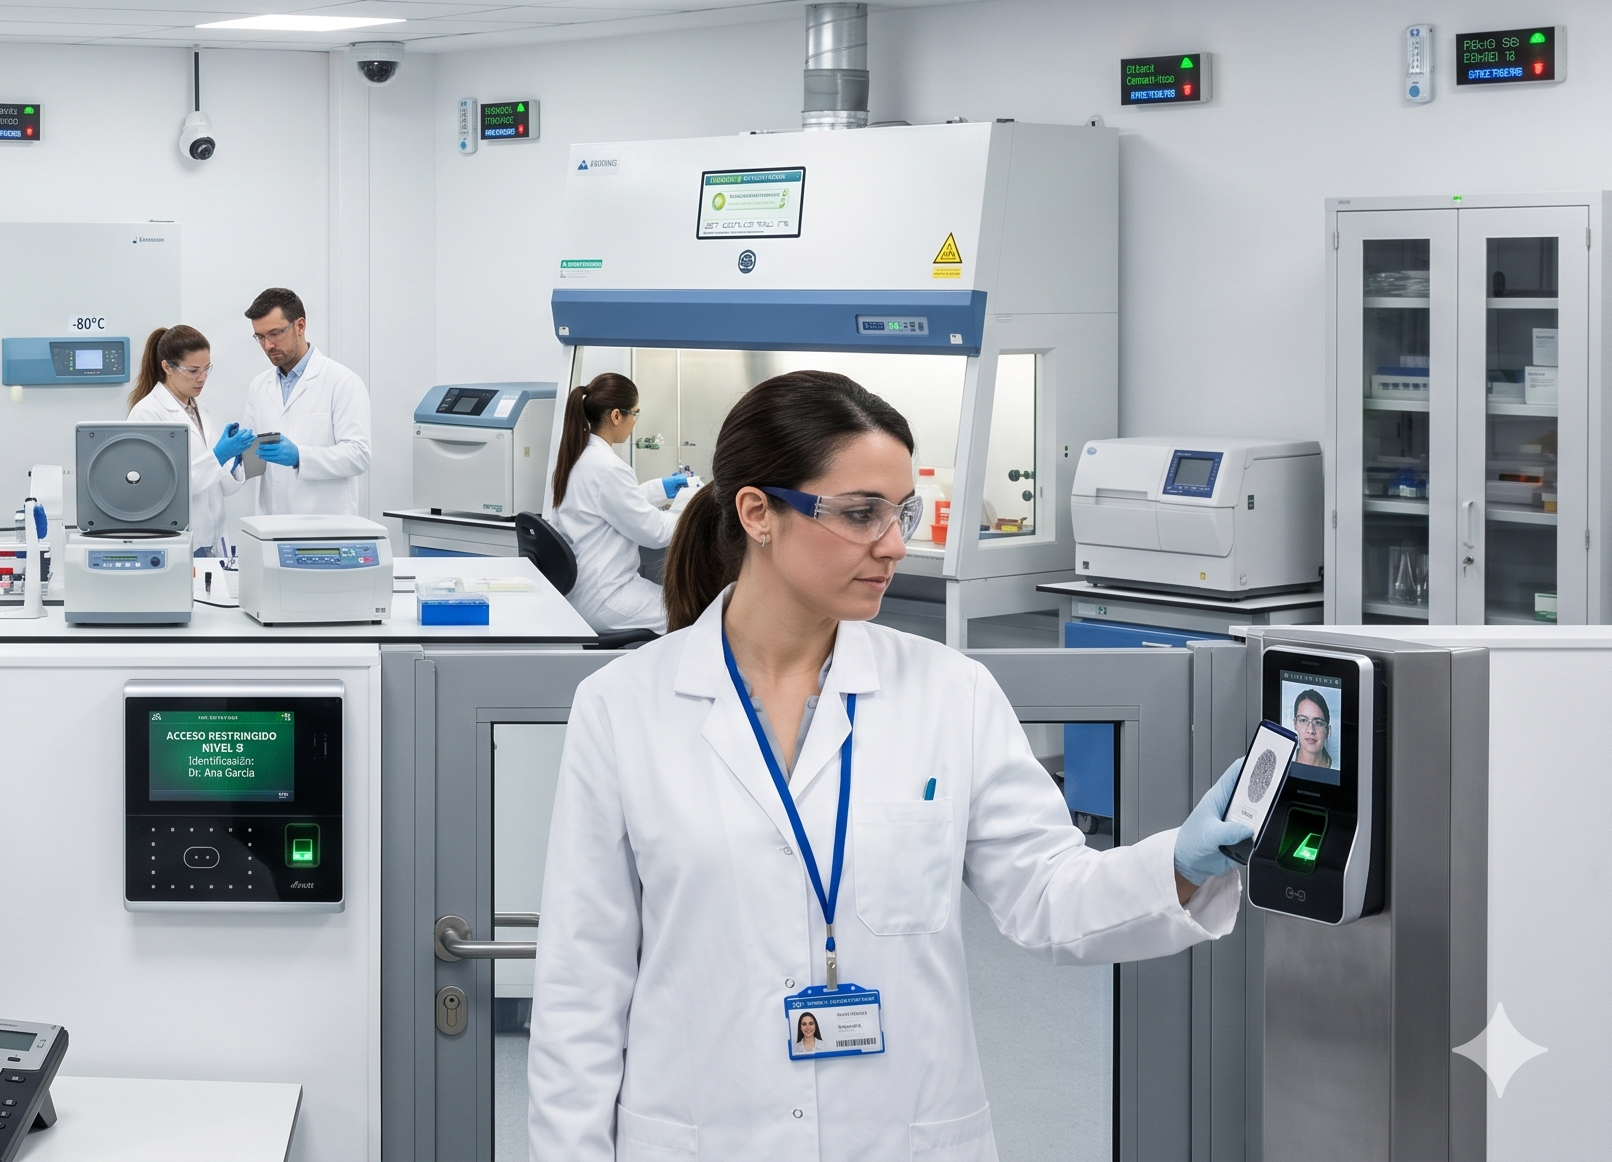
\includegraphics{images/title-page/labo1.png}};

    \end{tikzpicture}
\end{frame}